\documentclass[fontsize=12pt,paper=letter,cleardoublepage=plain]{scrbook}

% adapted from https://github.com/jonhoo/thesis/

% for 1.5 line spacing
\usepackage{setspace}
\onehalfspacing
% single spacing for table of contents
\AfterTOCHead{\singlespacing}

% recompute page layout based on the above
\recalctypearea

% more colors (like RedOrange)
\usepackage[dvipsnames]{xcolor}

% qualitative colors
% subset of https://jfly.uni-koeln.de/color/
% that is also distinctive in grayscale
\definecolor{set1}{HTML}{0071b2} % blue
\definecolor{set2}{HTML}{e59c00} % orange
\definecolor{set3}{HTML}{009e73} % green
\definecolor{set4}{HTML}{efe440} % yellow

% so we can splice in PDFs
\usepackage{pdfpages}

% set up bibliography
\usepackage[square,comma,numbers,sort&compress]{natbib}

% enumerate* and itemize*
\usepackage[inline]{enumitem}

% for \begin{comment}
\usepackage{verbatim}

% for source-code listings
\usepackage[newfloat,draft=false]{minted}

% for formulas
\usepackage{mathtools}

% to split lists into multiple columns
\usepackage{multicol}

% for "on page NN" reference
\usepackage[nospace]{varioref}

% for \sfrac
\usepackage{xfrac}

% for \ifoptionfinal
\usepackage{ifdraft}

\usepackage[breaklinks, pdfborder={0 0 0}]{hyperref}

% do not reset page numbers at \mainmatter
\let\mainmatterorig\mainmatter
\renewcommand\mainmatter
 {\edef\p{\arabic{page}}%
  \mainmatterorig
  % we need to compute the actual current page number. we know the page number
  % from _before_ we called \mainmatter. but what is it now? well, it is
  % certainly that +1. but we also need to account for the next chapter starting
  % on a "right" (odd) page. we do this by adding the page number modulo two.
  % TODO: double check before final version
  \setcounter{page}{\p+1+(\p-\p/2*2)}%
 }

% an environment for todos
\newenvironment{inprogress}
  {\vspace{.5em} \color{set2} \noindent \textbf{TODO}}
  {\vspace{.5em}}

% a command to indicate current editing progress
\newcommand{\resume}{
  \begin{center}
    \color{set2}
    \hrule
    \vspace{1pt}
    \hrule
    \hrule
    \vspace{10pt}
    \textbf{This section is not yet complete.}
    \vspace{10pt}
    \hrule
    \hrule
    \vspace{1pt}
    \hrule
  \end{center}
}

% an environment for invariants
\newcounter{invn}
\renewcommand{\theinvn}{\Roman{invn}}
\newenvironment{invariant}
  {\vspace{.5em} \color{set1} \refstepcounter{invn} \noindent \textbf{\color{set1} Invariant \Roman{invn}.}}
  {\vspace{.5em}}

% for handy reference
%
% paragraph without spacing:
% \setparsizes{0pt}{0pt}{0pt plus 1fil}

% in thesis: titlehead, subject, title, subtitle
\title{Verifying a concurrent, crash-safe file system}
\author{Tej Chajed}
\begin{document}

\frontmatter

% always arabic page numbering (default is roman in \frontmatter)
\pagenumbering{arabic}

\section*{Acknowledgments}
\begin{spacing}{1}
  \ifoptionfinal{\tej{write the acknowledgments}
}{Will be included in the final submission.}
\end{spacing}
\cleardoublepage

\section*{Prior Publication}
Parts of this thesis were previously published in a conference
paper~\cite{chajed:gojournal}.
\cleardoublepage

\tableofcontents

\mainmatter

\chapter{Introduction}%
\label{sec:introduction}

One crucial service in an operating system is its \emph{file system}, the
software that implements the abstraction of files and directories on top of a
disk, which simply stores a long sequence of bytes. File systems are important
because they are used by all applications to store data, and bugs in file
systems are especially costly because they can lead to data loss for any of
these applications. One approach to improve reliability is to use formal
verification, in which the file system is developed along with a proof that it
always follows a high-level specification of its intended behavior. This thesis
develops new techniques to address the key challenges in a file system of
reasoning about \emph{concurrency} and unexpected \emph{crashes} where the whole
computer reboots, a verified transaction system that handles these concerns, and
a file system that uses the transaction system. The final artifact is DaisyNFS,
a verified file system that comes with a proof of correctness and that achieves
good performance.

\section{Motivation}
\label{sec:intro:motivation}

A file system is an especially critical system for
three reasons. First, the file system is widely used --- essentially all applications have
data that is ultimately stored in a file system. Second, implementations are
concurrent and optimized, which increases the potential for bugs. Finally, bugs
are particularly costly since they can lead to permanent data loss for any
application running on top.

Two challenges make implementing a correct file system challenging: crashes and
concurrency. A file system is generally expected to keep application data safe
even if the system stops running at any time, say due to a power failure or
kernel panic. This thesis uses ``crash'' to refer to any of these circumstances
where the computer stops and is rebooted. After a reboot, the file system is
expected to preserve data from before the crash. The second big challenge is
concurrency in the implementation, which complicates approaches for improving
reliability, including both testing and verification.

Bugs are still discovered in widely used file systems like ext4 and btrfs,
despite a long history of developing, testing, and using these file systems. A
recent approach for fuzzing file systems~\cite{kim:hydra} found new crash-safety
issues in both ext4 and btrfs, despite not testing for concurrency issues. A
study conducted in 2013 looked at all patches for Linux file systems from
2005--2013~\cite{lu:fsstudy}, finding hundreds of these patches were to fix bugs
(for example, 450 for ext4 and 358 for btrfs). About 60\% of these bugs lead to
data loss or crash the kernel (and as the study points out, these are much more
serious consequences than most bugs in application software). File systems have
a lot of internal concurrency for performance reasons, which both leads to bugs
and makes testing and fuzzing more challenging.

The approach in this thesis to make a reliable file system is to use formal
verification. In this approach, we write the code, then a specification of the
intended behavior of the code, and finally a mathematical proof that shows the
code always meets the specification. For confidence in the proof itself, the
proof is carried out in a computer and a piece of software called a proof
assistant checks that the proof is valid. The nature of formal verification
forces the proof engineer to systematically cover every corner case in the code.
As a result, they can completely rule out whole classes of bugs, including
low-level bugs like memory safety but also logic errors like returning the wrong
data. Verification does not guarantee that a system is bug-free, because the
specification must be correct and the assumptions in the proof must hold in
practice, but it does help since the specification is smaller than the
implementation, and it isolates debugging to identifying where the specification
is wrong or an assumption was violated.

While the idea of formal verification is not new, there was essentially no
support for reasoning about the combination of crashes and concurrency when this
thesis work started (in 2015). Thus this thesis develops new techniques to
reason about the combination in the first place. We apply these techniques to
DaisyNFS, a verified implementation of the Network File System (NFS) protocol, a
standard file-system interface.

The key to verifying a system with the complexity of DaisyNFS is a design
that splits the file system into two main parts: a transaction system called
GoTxn that makes it easy to get atomicity over the disk, and then the rest of
the file system implemented using a transaction per operation. GoTxn must face
the key challenges of crash safety and concurrency, but it handles them in such
a way that the code on top is verified using comparatively much simpler
sequential reasoning. The file-system code then focuses on implementing features
like the details of the NFS semantics, large files, and efficient data
structures.

\section{State of the art}
\label{sec:intro:related}

Production file systems are generally validated by testing. While testing is
indispensable for development, the nature of a file system makes it difficult to
catch all bugs with only testing. The fundamental difficulty is a high degree of
non-determinism from two sources: crashes in the middle of execution, and
concurrency in the implementation that is needed for good performance.

The importance of file-system correctness has been recognized by the academic
community, thus there are many approaches for increasing confidence with
improved testing. One line of work has explored systematically testing crashes
at intermediate points~\cite{mohan:crashmonkey,pillai:appcrash,yang:explode}. Another line of
work has focused on fuzz testing as a way to induce crash-safety
bugs~\cite{xu:janus,kim:hydra}. These approaches have been successful for
finding bugs, including crash-safety bugs, but they only test sequential
executions, missing bugs due to concurrently issued operations or from crashes
that interrupt multiple operations. Furthermore, unlike formal verification, testing cannot
cover all executions of a program, even without crashes and concurrency,
potentially missing bugs.

The research community has also recognized the value of formal verification for
reasoning about a file-system implementation. The closest related work is
Flashix~\cite{bodenmuller:concurrent-flashix}, a verified, concurrent file
system that runs on flash devices. The techniques
developed to verify Flashix are specialized to its particular file-system
design, especially its write-back cache. Its concurrency is primarily between
regular operations and garbage collection, and read-only concurrency. This
thesis develops a general logic for reasoning about crashes and concurrency and
applies this logic to verify a system with write-write concurrency.

There are other verified file systems, especially the sequential file systems
FSCQ~\cite{chen:fscq} and Yggdrasil~\cite{sigurbjarnarson:yggdrasil} and an
concurrent but in-memory file system AtomFS~\cite{zou:atomfs}. These systems use
verification techniques that do not support both crashes and concurrency, and they
cannot be extended them in a straightforward way to support the other form of reasoning.

\section{Approach}
\label{sec:intro:approach}

What does it mean to give a machine checked, formal proof of a system? At a high
level, program proofs always have three components: an implementation, a
specification, and a proof. When doing machine-checked proofs, all three are
physically represented as code in a verification system. The verification system
checks the proof against the implementation and specification, ensuring that the
proof is complete.

This thesis integrates interactive, foundational proofs using custom
infrastructure (in Coq) as well as automated verification using a
verification-aware programming language (Dafny). These are both machine-checked,
formal proofs, but the interaction models of the two systems are different
enough that this section describes them separately.

In Coq, the core feature is proofs based on dependent type theory, which is
expressive enough to represent essentially any math. A first step when using Coq
is to connect the code to the reasoning in the proof assistant. The particular
approach in this thesis translates executable code to a model in Coq,
implemented by a tool called Goose. The model
and its semantics encodes the
assumptions the proof makes about how the program behaves. The semantics is typically structured as a transition
system, where an execution is a sequence of states the program goes through
along with some notion of observable behavior, like external I/O or return
values. \tej{maybe add a figure of an execution trace}

Once we have a program in Coq, we can reason about it. The goal of
verification is to prove that the program meets its specification, and
where the specification describes the allowed behaviors of the program. The
specifications in this work forbid universally incorrect behavior, like reading an
out-of-bounds address in an array, but more precisely specify what the program
is supposed to do, for example how it responds to user requests.

A common structure to tame the complexity of reasoning about a program is to use
a \emph{program logic}. In principle it might be possible to prove a theorem
about all the behaviors of a program directly, but such a proof would too
complex to be feasible. The program logic organizes the proof with a structured
way of expressing and proving statements about the program, such as breaking the
proof down into theorems about individual functions. The proof in a program
logic will often mirror the structure of the code, since each function has its
own specification and groups of related functions have related specs.

Program logics for concurrency are still an active area of research; only
recently have they reached the maturity to give completely mechanized proofs of
moderate-sized programs. There are few logics that also can reason about crash
safety. Our approach in this thesis is to build a new program logic called Perennial with all the
concurrency-reasoning features of a modern program logic, plus new features for
reasoning about crashes. What makes this feasible is Iris, a modular framework
for concurrency. Iris includes a concurrent program logic which we are able to
extend with crash-safety reasoning while preserving the concurrency reasoning
features, without reimplementing them from scratch.

Using our new program logic, we verified GoTxn, a concurrent transaction system.
The transaction system's correctness theorem says that any program that uses
transactions really has transactional behavior: its execution is equivalent to a
version of the program where the transactions run atomically. The complete
specification includes some important details in order to formalize the
intuition behind atomicity.

Next, because transactions appear to run sequentially, and write to disk all at
once, it is no longer necessary to use a sophisticated program logic like
Perennial to reason about the body of each transaction. Instead, we switch to
using Dafny, a verification-oriented programming language that only supports
sequential code but as a result is highly productive for this use case. The file
system is written and verified in Dafny, then compiled to Go and linked with
GoTxn.

Dafny verification works quite differently from Coq. Dafny is a programming
language with verification features; contrast this with Coq, which supports
general math that can \emph{model} programs. A Dafny method can be annotated
with a specification. The Dafny checker converts a method and its specification
to a logical formula (called a verification condition), which is true if and only if the specification holds for
the method. It then queries a \emph{solver} (Z3, in the case of Dafny) to determine if the formula is true.
Contrast all of this with Coq, where the user manually develops the program
logic and connects the rules of this logic. Checking a program against its specification in Dafny cannot be perfectly
automated because it is impossible to answer whether a general logical formula
is true or not, but the user can insert annotations to help out the solver, and
generally fewer annotations are needed than lines of proof for Coq. The main
downside to this approach is that it fixes a sequential programming language, so
unlike in Coq, it isn't possible to reason about concurrency and crashes.

\Cref{fig:overview} depicts how all of the components of DaisyNFS and its proof
fit together. The left-hand side depicts the implementation, split between GoTxn
and the file-system implemented in Dafny. The Dafny code is compiled to Go and
then the two parts are linked together into one \cc{daisy-nfsd} binary in the
usual Go build process. GoTxn is translated to a model using a tool called
Goose. The right-hand side of the figure depicts all aspects related to the
proof, which is written using the Perennial program logic. All of this happens
in the Coq proof assistant, which checks that the proofs are valid. Meanwhile
the DaisyNFS file-system code is verified in Dafny, which integrates
implementing, specifying, and verifying code. This proof is checked by the Dafny
verifier. Finally, the proof of GoTxn is written in such a way that it can be
composed with the proof of DaisyNFS for a theorem about the whole
\cc{daisy-nfsd} binary. This is a conceptual composition, not one in either
Dafny or Coq.

\begin{figure}[ht]
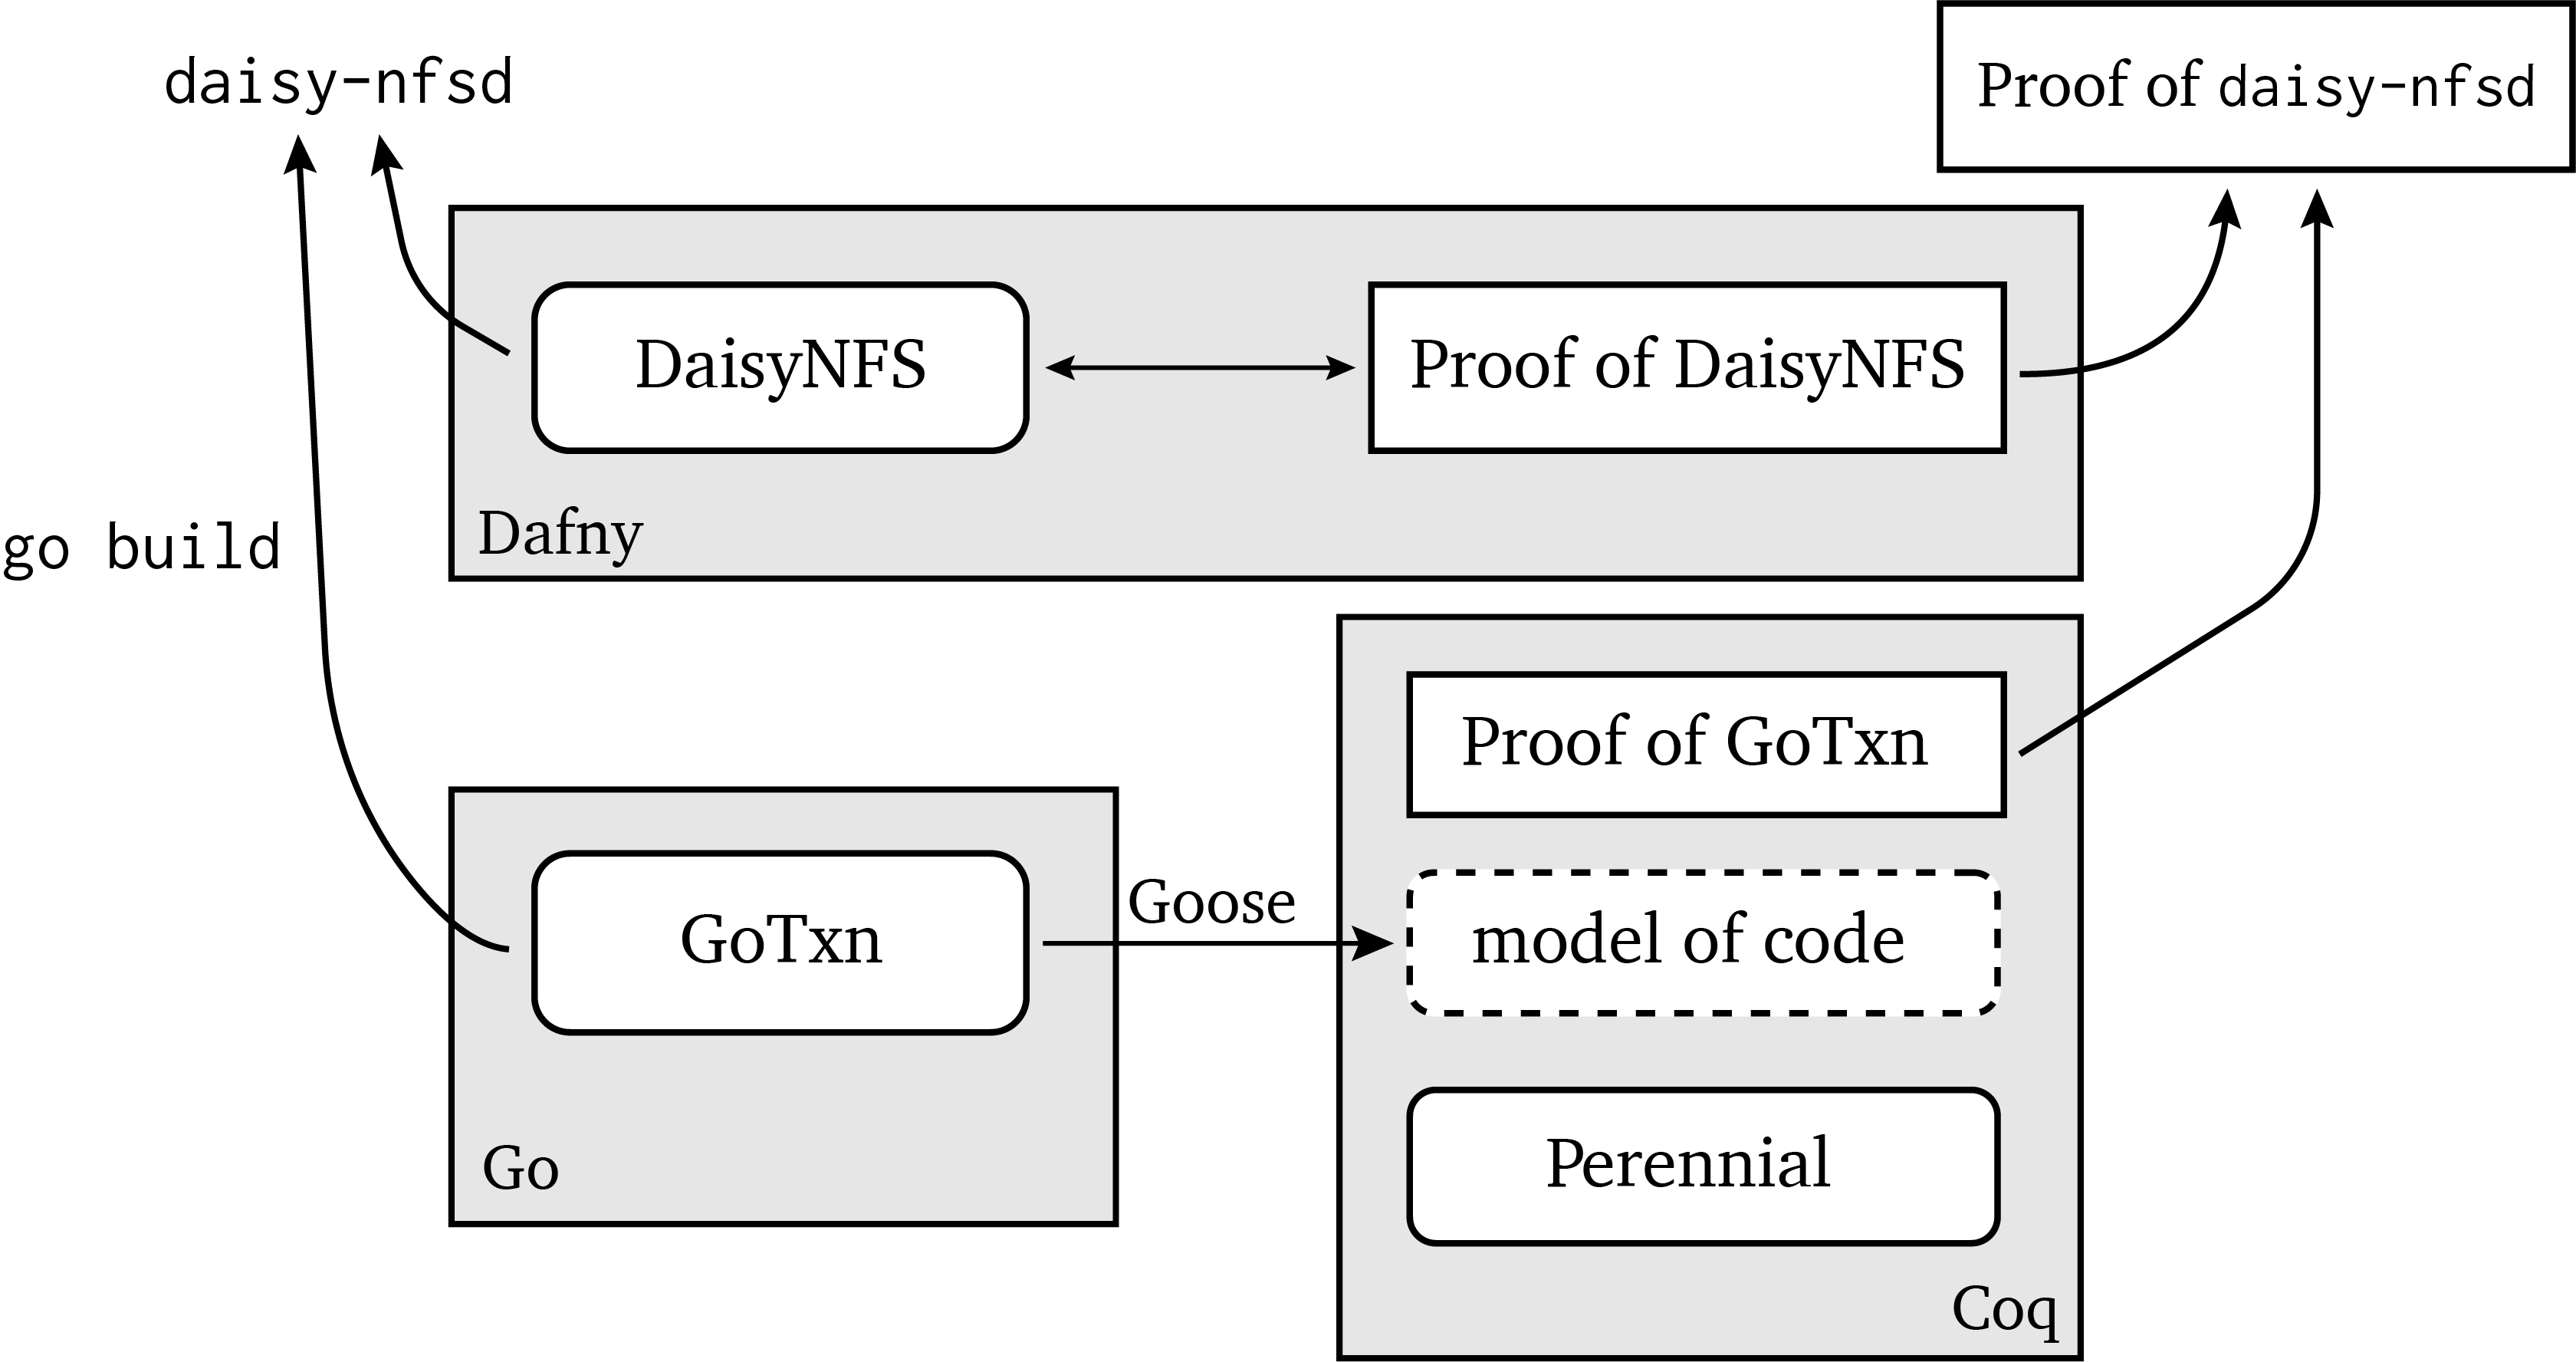
\includegraphics{fig/overview.png}
\caption{Overview of how GoTxn, DaisyNFS, and the proofs fit together.}
\label{fig:overview}
\end{figure}

One of the contributions of this thesis is that the file-system design isolates
concurrency and crash safety into the transaction system. This structure leaves
the rest of the implementation only to \emph{sequentially} implement the
file-system logic and data structures. Because this is sequential, crash-free
execution, we use Dafny to implement and verify each operation, then run this
code wrapped in a transaction. Intuitively what the file-system proof shows is
that it correctly implements the NFS protocol.

In order to connect the file system's sequential proofs to its concurrent
execution, we prove a general theorem about the transaction system's
implementation. The starting point is the idea of a \emph{simulation} proof,
which shows that a system like the file-system transactions correctly implement an
abstract specification like the NFS protocol. The GoTxn
\emph{simulation-transfer theorem} shows that for any system implemented using
transactions with a sequential simulation proof, the concurrent system running
with GoTxn concurrently simulates its abstract specification where each
operation is atomic. Intuitively this theorem holds because every concurrent
execution of the GoTxn transactions appears to be atomic, and then the
sequential simulation proof shows those atomic transactions implement the
abstract specification. However, the GoTxn theorem formalizes precisely what
conditions are required for the simulation transfer, including restrictions on
the transactions and exactly what crash safety guarantees are achieved.

\section{What is the value of verifying a file system?}

The reader might wonder what the value of this kind of large verification effort
is.

\paragraph{Cost versus benefit.} There are many less formal ways to make
software more reliable, including testing, fuzzing, and code auditing. Formal
verification also has a spectrum; we could potentially apply property-based
testing, model checking, or symbolic execution to parts of the code. Rather than
verifying the implementation, we could instead attempt to model and specify key
parts of the algorithms or system design, then verify those. What is the
additional value of fully machine-checked proofs, all the way down to the code?

Verification in the real world needs to have benefits that outweigh the costs.
The benefit of reliability for file systems is hopefully clear, from the
exposition above. I see this work as lowering the cost of verifying crash-safe
and concurrent systems: formerly, there simply didn't exist techniques for this
kind of proof, and now it is possible (and at least the cost is bounded by a PhD
thesis and not something much larger). Building on these foundations, I hope the
costs come down to make verification an appealing alternative to verification
for the next generation of storage systems.

The real ideal for verification is not just it is worth paying the costs but
that verification enables something that would otherwise not be doable. With
file systems I believe this is possible, since verification might enable a new
file system with more daring optimizations to gain confidence faster than would
otherwise be possible. There aren't that many widely-used file systems --- most
people use one of ext4, btrfs, or XFS on Linux, NTFS on Windows, and APFS on
macOS --- and new file systems are generally adopted very slowly. APFS was
surprising for having only a 3-year development period before Apply widely
deployed it, and this was probably only possible because of Apple's tight
vertical integration. Ext4 is the other ``new'' file system, introduced in 2008
(by extending ext3, which was first released in 2001).

% ext4: 2008
% ext3: 2001
% XFS: 1994 (first released on IRIX OS for SGI)
% NTFS: 1993
% APFS: 2017

\paragraph{Verification guides debugging.} With a verified system, bugs are
still inevitable since there is unverified code surrounding the verified code,
the assumptions of the proof can be violated, and the specification can be
wrong. However, an advantage of formal verification, particularly fully
machine-checked proofs, is that when bugs are discovered it's safe to start
debugging with all the code outside the verification as well as looking at the
specification.

\resume

\section{Contributions}
\label{sec:intro:contributions}

This thesis makes the following contributions that enable its overall goal of a
verified, concurrent file system:

\begin{itemize}
  \item \textbf{Perennial} is a program logic for crash safety
        and concurrency using specifications based on crash weakest
        preconditions. These include crash conditions combined with concurrency
        and reasoning principles for moving ownership to a recovery procedure
        following a crash. \textbf{Logically atomic crash specifications} are a
        pattern using Perennial's crash weakest preconditions for specifying
        libraries that have both concurrent behavior and involve persistent
        state. These are implemented using Perennial and used in the GoTxn
        proof.
  \item GoTxn has a new \textbf{lifting-based specification} for its journaling
        layer to reason about concurrent transactions separately, which is
        challenging since the logical disk can change in the middle of a transaction. Its proof uses a novel
        \textbf{history-based abstract state} for the write-ahead log. This model allowed us to carry
        out a modular proof where the write-ahead logging library hides most of
        its internal complexity, simplifying reasoning about the rest of the GoTxn
        code that uses it. Finally, GoTxn exports a \textbf{program refinement}
        specification that captures how transactions appear to run atomically.
  \item DaisyNFS uses a \textbf{simulation-transfer theorem}, proven on top of
        GoTxn's program refinement specification, which shows that sequential
        reasoning for each transaction in a system implies correctness for the
        whole system when run on top of GoTxn. This justifies using Dafny, a
        sequential verification language, to verify the DaisyNFS implementation.
        The specification for DaisyNFS uses a mathematical formulation of RFC
        1813, the document that (in prose) specifies what a NFSv3 server should
        do.
  \item \textbf{Goose} connects efficient code implemented in Go to a model of
        that code in Perennial. A general contribution here is a design for
        systems verification that enables efficient code and convenient
        reasoning. Goose includes reasoning principles for the models that it
        outputs, to support verifying the translated code.
\end{itemize}

The ideas in Perennial and Goose are applied to GoTxn, but they could be used
for reasoning about other concurrent storage systems. Similarly,
this thesis applied GoTxn to a verified file system, but it could also be used
as the basis for other verified storage systems, like a persistent key-value
store.

\tej{describe limitations at a high level}

\section{Reading guide for the thesis}
\label{sec:intro:reading-guide}

This section briefly outlines the chapters of the thesis, the dependencies
between chapters, and the intended audience. Broadly the thesis is intended for
a systems audience, except for the verification foundations. The support for
concurrency makes all of the formal underpinnings in the thesis more technical
than foundations for sequential systems verification.

\Cref{ch:related} covers related work across Perennial, GoTxn, and DaisyNFS, for
a broad computer-science audience. To keep the Goose chapter self-contained, its
related work is described in the relevant chapter.

\Cref{ch:perennial} is an overview of Perennial. This chapter is oriented
towards a reader interested in the general verification concepts and not
necessarily the systems side. At this level of abstraction Perennial is
independent of both the GoTxn proof and even Goose for verifying Go code. Some
experience with program logics is helpful for understanding the presentation.

\Cref{ch:crash-logatom} describes a style of logically atomic specifications
that capture both concurrency and crash atomicity using Perennial. It uses an
extended example from the GoTxn proof and explains its formal underpinnings at a
high level. This is the most technically involved chapter.

\Cref{ch:txn} describes the design and proof of GoTxn. An important part of GoTxn is its
specification, which captures how transactions are atomic. This chapter does not
require the full Perennial or logical atomicity chapters.

\Cref{ch:daisy-nfs} describes the design and proof of DaisyNFS.\@ This chapter
explains the proof approach that justifies using Dafny to verify DaisyNFS even
though Dafny is a sequential verification tool and DaisyNFS is a concurrent
system.

\Cref{ch:goose} is about Goose and talks about verifying Go code generally, with
nothing specific to GoTxn or even storage systems. This is the first detailed
description of Goose, so this chapter is written to be readable without any of
the other chapters.

\Cref{ch:impl} is a short chapter covering some implementation details in
DaisyNFS, covering both GoTxn and the file-system code.

\Cref{ch:eval} evaluates the whole file system along a few dimensions,
especially performance but also aspects of the proof.


\chapter{Related Work}
\label{sec:related}

While verifying programs is an old idea, going back at least to Floyd and
Hoare's work in the late 1960s~\cite{floyd:meanings,hoare:logic}, prior to this
thesis (in 2015) there was almost no work on reasoning about a program's
execution in the presence of a crash, let alone the combination of concurrency
and crashes. The full pipeline of systems verification is also quite new:
connecting the formal reasoning to executable programs, writing machine-checked proofs, and scaling up the techniques to
systems with sizable implementations.

The Perennial framework for reasoning about crashes and concurrency draws on two
lines of research: sequential crash safety verification and concurrency
verification, described in
\cref{sec:rel:crashes,sec:rel:concurrency,sec:rel:crashes-concurrency}. DaisyNFS
draws from two other lines of prior work, on verified transactions and file
systems, described in \cref{sec:rel:verified-fs,sec:rel:verified-txn}.

The most closely related work is Flashix, another verified concurrent and
crash-safe file system. \Cref{sec:rel:flashix} compares the two systems'
contributions and results. Finally, \cref{sec:rel:txn} discusses some related work
on using transactions as part of a file system.


\section{Foundations for verifying sequential crash safety}
\label{sec:rel:crashes}

There are a variety of foundational tools for reasoning about crash safety,
largely for sequential systems.

FSCQ~\cite{chen:fscq,chen:dfscq,hchen-phd} is a sequential file
system verified with Crash Hoare Logic (CHL). CHL's basic specifications have
the form $\hoareC{P}{e}{Q}{Q_{c}}$, extending the Hoare triple $\hoare{P}{e}{Q}$
with a \emph{crash condition} $Q_{c}$ that holds at all intermediate points in the
function's execution. Crash conditions handle a core difficulty of crashes,
namely that they stop the system at some intermediate step. There are two
remaining challenges: a crash wipes in-memory state, and the system might crash again
while recovering after a crash. CHL connects the system's crash conditions to a
specification for recovery to handle these two issues. A crash predicate
transformation captures what can be assumed when recovery starts, and for
crashes during recovery CHL requires that recovery be \emph{idempotent} in the
sense that its crash condition implies its own precondition. CHL was used to
specify and verify FSCQ~\cite{chen:fscq} and a more performant successor
DFSCQ~\cite{chen:dfscq}.

Yggdrasil~\cite{sigurbjarnarson:yggdrasil} takes a different approach to crash
safety. The basic definition is \emph{crash refinement}, which says that a
system implements an interface correctly, including a specification for what a
crash followed by recovery is allowed to do. Note that unlike CHL this
specification is about a collection of methods implementing an abstract,
specification transition system, not about individual methods. Yggdrasil uses
crash refinement to specify and verify a file system comparable to the file
system in xv6, a teaching operating system. The implementation uses Z3 to check
crash refinement, which the authors show is able to handle a system of this
complexity by breaking down the implementation into small enough layers.

Argosy~\cite{chajed:argosy}, which I led the development of but is not part of
this thesis, combines aspects of FSCQ and Yggdrasil. The key new idea is to
develop the metatheory for \emph{recovery refinement} that shows how systems
compose when both have recovery procedures --- what is non-trivial to handle is
that a crash in the composed recovery procedure requires starting over from the
beginning. Recovery refinement can be viewed as an extension of crash refinement
with verified metatheory for recovery, largely left implicit in the Yggdrasil
paper. Argosy also shows how to encode the conditions of recovery refinement
using CHL so that a single layer is verified using the CHL program logic.

VeriBetrKV~\cite{hance:veribetrkv} takes yet another approach to reasoning about
crashes, this time friendly to encoding in Dafny, a sequential verification
system with integrated support for programming and verification. The main idea
related to crash safety is to adopt the style from
IronFleet~\cite{hawblitzel:ironfleet} and think of a storage system as a
distributed system made up of the CPU and the storage device. The extension
needed for crash reasoning is to add a crash transition to the storage device
that non-deterministically wipes any buffered but unacknowledged writes, and
then to show that when this happens it corresponds to an appropriate
application-level transition modeling crashes (similar to the crash refinement
definition from Yggdrasil and recovery refinement in Argosy, although this is
associated with a code transition rather than a dedicated recovery procedure).
VeriBetrKV is used to verify a persistent key-value store based on
B\textsuperscript{$\epsilon$} trees, a data structure that also underlies
BetrFS~\cite{jannen:betrfs}.

Perennial has crash conditions that look similar to CHL's crash conditions,
albeit as part of a concurrent program logic rather than a sequential one. We do
carry out a refinement proof in the style of Argosy, which is similar to the
specification style in VeriBetrKV and Yggdrasil, but because it is connected to
concurrent reasoning the proof techniques are more sophisticated.

\section{Foundations for verifying concurrent programs}
\label{sec:rel:concurrency}

There are a number of approaches proposed to verifying concurrent programs, and
Iris in particular is the basis for Perennial. It
would be hard to do justice to the historical development of concurrency
reasoning. Looking at approaches that are actively used in research and
connected to executable implementation, two broad strategies are commonly used:
developing concurrent \emph{program logics}, and using \emph{refinement}-based
techniques.

Many refinement-based techniques are based on the idea of \emph{reduction},
which appeared originally in Lipton's theory of ``movers''~\cite{lipton:movers}.
The idea behind reduction is to reason about a program through program
transformations that show the program is equivalent to a simpler program. These
techniques can reason about concurrency by showing that a concurrent program is
equivalent to a program with sequential or atomic regions. These ideas have been
used as part of the CIVL verifier~\cite{hawblitzel:civl,kragl:civl-layers} and
Armada~\cite{lorch:armada}; my own prior work on CSPEC~\cite{chajed:cspec} was
also based on movers, before starting Perennial. Reduction-based techniques
generally reason about a program through a series of transformations, each
making the program slightly simpler, keeping the proof of each transformation's
correctness more manageable.

One large verified system, CertiKOS, is based on a custom verification
infrastructure called Certified Concurrent Abstraction
Layers~\cite{gu:certikos-ccal} which based on refinement but not reduction. This
work is notable for verifying a system (a simple operating system) not just at
an abstract protocol level but all the way down to concurrent code. The proof
composes with the CompCert compiler correctness theorem to carry the guarantees
down to the assembly code of the operating system.

Program logics are an alternative approach based on giving specifications to
each function in the program, within a logic that has useful rules for proving
and composing specifications. Hoare logic is a classic program
logic for sequential programs that based on pre- and post-conditions.
Concurrency makes it harder to construct a logic that can usefully reason about
many concurrency patterns (completeness) while also giving specifications that
hold in the presence of concurrent threads (soundness). One productive line of
work has been based on concurrent separation logic (CSL)~\cite{brookes:csl}.

The Verified Software Toolchain is notable for connecting a CSL-based logic
(VST-Floyd) down to proofs of C code, including a connection to CompCert to
carry these guarantees down to assembly~\cite{cao:vst-floyd}. It has been used
for a number of sequential verified C programs and recently to some shared
memory C libraries.

Microsoft VCC~\cite{cohen:vcc,cohen:vcc-local} is another verification system
that is based on annotating C code with pre- and post-conditions and so-called
two-state invariants that are similar to rely-guarantee
reasoning~\cite{jones:rg,feng:lrg}. VCC is typically used to encode a form
of concurrent refinement reasoning while also using specifications similar to
that of a program logic. The system was used to verify a portion of Hyper-V. The
system is implemented as a verification-condition generator; unlike the program
logics described in this section, VCC has no soundness argument (even on paper)
to specify what its specifications mean and argue that it enforces the right
conditions for that meaning to hold.

Perennial builds directly on Iris~\cite{jung:iris-jfp}. Iris is a general
framework for concurrency, featuring a base logic with key features for
concurrency (step indexing and separation-logic resources, including
\emph{higher-order} resources used to define invariants for example) and a
program logic built on the base logic. This decomposition was valuable for
Perennial because we made two core changes to Iris: first, the program logic
itself is extended with crash safety reasoning, and second, the framework is
applied to our GooseLang models of Go code. In both cases the generality of Iris
was valuable, as the framework is not tied to reasoning about a particular
programming language or even to its usual program logic. Prior to this work,
Iris had not typically been used for reasoning about executable code (though
projects like RefinedC~\cite{sammler:refinedc} and our own work on Goose are
changing that).

\section{Reasoning about crashes and concurrency}
\label{sec:rel:crashes-concurrency}

Program logics other than Perennial have been developed for formal reasoning
about concurrent, crash-safe systems. Fault-Tolerant Concurrent Separation Logic
(FTCSL)~\cite{ntzik:faults} extends the Views~\cite{dinsdale:views} concurrency
logic to incorporate crash-safety. POG~\cite{raad:pog} is a program logic for
reasoning about the interaction of x86-TSO weak-memory consistency and
non-volatile memory. Both of these logics are only defined on paper, and do not
support mechanized proof. Perennial goes beyond their reasoning principles: it
includes ownership reasoning and its interaction with crashes, and a style of
logically atomic crash specifications for modularly specifying libraries and
composing their proofs. FTCSL and POG have no mechanism of modular proofs of
layers, which we found essential to scale verification to a file system.

In the case of x86-TSO with persistence, POG required a line of research to
define the semantics at the
ISA level, validating this semantics against the hardware and in conversations
with Intel engineers~\cite{raad:px86,raad:px86-extended}. A similar semantics effort defines the
semantics of ext4 under crashes, but without an accompanying program
logic~\cite{kokologiannakis:persevere}. It would be an interesting direction for
future work to combine the persistency semantics of x86 with Perennial, to
verify libraries that use non-volatile memory.

\section{Verified transaction systems}
\label{sec:rel:verified-txn}

As far as we know, GoTxn is the first transaction system that makes data durable
and has a verified implementation. There is much related work on verifying
aspects of transaction systems with and without durability, and on unverified
transaction systems.

\citet{ChkliaevHS99} verify serializability of two-phase locking and other
transaction concurrency control mechanisms in the PVS theorem prover. Their
proof formalizes two-phase locking as an abstract protocol consisting of
sequences of read, write, and locking operations, as opposed to a concrete
implementation as in GoTxn. \citet{pollak-2PL} uses a variant of the
CAP separation logic~\citep{dinsdale:cap} to give a pen-and-paper
proof of serializability for an abstract, protocol-level description of
two-phase locking, connecting the protocol to atomic reasoning about
transactions.

\citet{mohsen:stm} developed a framework for verifying software transactional memory algorithms, modeled
as I/O automata. They applied their framework to sophisticated STM algorithms, such as
NOrec algorithm~\cite{dalessandro:norec}. The STM algorithms considered do not
handle persistence, so the framework does not address crash-safety reasoning.

A specification called the Push/Pull model of
transactions~\cite{koskinen:pushpull} is similar to the \emph{lifting} technique
in the journal system's specification~(\cref{sec:txn:lifting}) --- the core
problem addressed is that a journal operation atomically modifies a small number
of objects, but other objects can change between the start of the operation and when
it commits. The Push/Pull model also discusses reasoning on top of the
specification, using Lipton's reduction~\cite{lipton:movers} rather than
separation-logic ownership to handle concurrency. However that work is about
on-paper specifications and proofs, while we also prove an implementation meets
our specification and proved DaisyNFS on top.

DFSCQ~\cite{chen:dfscq} verifies a high-performance file system built on top of
a logging system with asynchronous disks and log-bypass writes, which are
challenging optimizations that GoTxn does not support. ARIES is a database
write-ahead logging protocol that was verified (with a pen-and-paper proof) in
FTCSL~\cite{ntzik:faults}; it is more sophisticated than GoTxn's write-ahead log
in that it can both undo and redo operations.

An important but unverified journaling system is jbd2, the ``journaling block
device'' that underpins ext3 and ext4 in Linux. The design of jbd2 is broadly
similar to that of GoTxn's journaling layer; GoTxn goes one step further and
also has automatic locking for transactions. One difference in the interfaces of
GoTxn and jbd2 is that in jbd2, transactions can reserve space ahead of time.
This has the benefit that a transaction can start writing to the journal on disk
while it is being prepared, potentially improving performance, but it also means
that a concurrent transaction must wait for all previously started transactions
to finish before becoming persistent, since a journaled operation can only be
logically completed when all prior operations are finished. This is a reasonable
tradeoff for a file system since transactions are generally short-lived, but it
sacrifices a bit of tail latency when an operation must be persisted, for
example when an application issues an \cc{fsync()}.

\section{Verified file systems}
\label{sec:rel:verified-fs}

The Dafny side of DaisyNFS is a new implementation but its design and aspects of
the proof strategy were inspired by other verified file systems like
DFSCQ~\cite{chen:dfscq} (especially its indirect block implementation described
in Alex Konradi's master's thesis~\cite{akonradi-meng}) and
Yggdrasil~\cite{sigurbjarnarson:yggdrasil}.

AtomFS~\cite{zou:atomfs} is a verified, concurrent file system, but its
implementation does not store data durably. The proof structure is quite
different from DaisyNFS in that all of the concurrency reasoning is part of the
file-system operations and there is no interaction between persistence and
concurrency. AtomFS is verified using a relational logic with rely-guarantee
reasoning; unlike separation logic, the basic specification in this logic is a
refinement statement that relates an implementation to a (simpler) specification
program.

We chose to verify an NFS server because it is widely used in practice and the
expected behavior of NFS operations is well documented in RFCs. FUSE is an
alternative for implementing file systems in user space that was used for the
verified file systems mentioned above, but its operations have a less clear
specification. FUSE also increases the trusted code to include both the FUSE
kernel component and the user-space library that connects the implementation to
the kernel.

\section{The Flashix file system}
\label{sec:rel:flashix}

The Flashix project deserves special attention since it also develops a verified
concurrent and crash-safe file system~\cite{bodenmuller:concurrent-flashix}.
Flashix targets flash storage, a lower-level storage technology than the drives
that DaisyNFS targets. The project has different goals around concurrency,
extending a sequential verified file system with limited concurrency. Flashix
has an idiosyncratic approach to reasoning about concurrency and crashes
specific to their file-system design, as opposed to Perennial's general
reasoning principles. Flashix is implemented using abstract data types in a
high-level language; a code generator transforms this code into executable C,
but this process is both not verified and has difficulty producing the most
efficient code using in-place updates.

While Flashix does have mechanized proofs, the approaches for both concurrency
and crash safety are layered on top in such a way that the top-level
specification and proof are not entirely within the proof assistant. Perennial
on the other hand formalizes the complete specification down to a simple
semantics for crashes and concurrency. Flashix also effectively has crash
reasoning throughout the system, whereas DaisyNFS factors out this reasoning to
GoTxn and then layers sequential proofs on top.

The Flashix project reports that components ``intertwined'' and could not be
separated as cleanly for reasoning purposes as they would have
liked~\cite[\S 8]{bodenmuller:concurrent-flashix}.
We had a similar experience within the transaction system, where
performance constrained the APIs of internal layers and forced us to export
complicated APIs. The  GoTxn was perhaps trickier than the components of Flashix
because we model code at a lower level of abstraction, so even issues like
concurrency and memory safety show up in each interface. We were inspired to
develop the DaisyNFS design to get truly sequential reasoning from the
experience of working in Perennial compared to automated verification in \fstar
and Dafny, and found modularity and clean abstractions much easier once
code ran within a transaction.

Where it lacks in generality, Flashix does make up for in verifying a taller
storage stack than DaisyNFS. Flash storage has a more limited API than a
standard drive --- in particular flash blocks must be completely erased before
being reused. A flash file system works around this limitation with \emph{garbage
collection}, where occasionally the system identifies a mostly-unused block,
moves its valid data elsewhere, and then erases it to reclaim space. This is
implemented by maintaining a logical-to-physical block mapping, similar to
virtual memory. DaisyNFS does not require any of this code, since we run on
devices that internally implement these features.


\section{Transactions to simplify system design}
\label{sec:rel:txn}

To be conducive to verification, DaisyNFS is implemented differently than
many NFS servers; in particular using two-phase locking is not common
practice.  Other user-level NFS servers are typically implemented on
top of an existing file system, relying on the underlying file system
for logging and locking. Ext3 and ext4 use a journaling system underneath, but
the file system and VFS layers perform locking. This locking is inherited when
these file systems are exported with the Linux NFS server. WAFL~\cite{wafl:hitz}
is an NFS appliance that provides snapshots and logs NFS requests to
NVRAM.\@  It has evolved its locking plan to obtain good
parallelism~\cite{curtis:wafl}.  Both the Linux NFS server and WAFL
are more complicated and have more features than DaisyNFS.\@

Isotope~\cite{shin:isotope} is a block-level transaction system similar to GoTxn
in its API, but without formal verification, which was used to implement a file
system called IsoFS. Its logging design is based on
multi-version concurrency control (MVCC) rather than our use of pessimistic
locking. The Isotope paper uses Isotope not only for the IsoFS file system but
also two persistent key-value stores. While GoTxn is in principle also suitable to implement a
key-value store, we have so far only used it in combination with DaisyNFS.\@

IsoFS has a similar design to DaisyNFS: it factors out isolation and atomicity to the transaction
system, making it easy to handle crashes and concurrency. Unlike GoTxn and
DaisyNFS, Isotope is still prone to subtle concurrency bugs in the transaction
system and bugs in the IsoFS code, whereas we use this split design to verify
both the transaction system and file-system code. The transaction API provided
by Isotope has an interesting performance optimization that GoTxn could support:
the API includes a \cc{please_cache} call that keeps an address in the
transaction system's cache, used for small but frequently-accessed metadata like
the allocator state in the file system.


\chapter{Goose}
\label{sec:goose}

A key component of any infrastructure for systems verification is the connection
between the proof and the executable code. The rest of this thesis focuses on
crash safety and concurrency as challenges to reasoning about storage systems.
This chapter is about Goose, which solves a more fundamental and practical
problem of reasoning about efficient code.

The basic setup we take for Goose is to first write the implementation in
ordinary Go, automatically translate the code to a model in the Coq proof
assistant, then carry out the proof on top of the model. Goose encompasses is
the entire process: it includes the translation tool itself, the way we model Go
code, and finally the reasoning principles for proving properties of translated
Go. (We will also use ``Goose'' in some places to refer to the subset of Go
supported by the translation tool.)

This chapter is intentionally fairly independent of the rest of the thesis for a
reader interested in verifying Go code but not the specifics of the
transaction-system proof or the file system built on top. Concurrency is
relevant to accurately modeling and reasoning about Go, but crash safety is also
of little importance in this chapter. Crashes are modeled simply by stopping
execution and wiping out all of the state except for the disk, which does not
relate to the specifics of Go.

\section{Goals and motivation}

There are two main goals for Goose: \textbf{flexibility} in writing code and
\textbf{soundness}. Flexibility is a goal so that the developer can write
efficient, high-performance code, as long as the proof engineer can also reason
about it (in this thesis the developer and proof engineer are frequently the
same). Goose is sound if the model captures the behaviors of the code, which is
required for the proofs to say something meaningful about the executable Go
code. If the code could go wrong in some way that the model doesn't capture, we
might finish a correctness proof but still have a bug; soundness makes sure this
doesn't happen.

There are alternate setups for verification where the connection between the
proofs and the code is not given by a model and translation, but the Goose
approach prioritizes flexibility in order to write fast code. The transaction
system sometimes does something efficient to shave off a bit of time, and its
proof pays the price by including a more complex correctness argument.

Soundness isn't a property we can immediately measure, since the translation
might miss subtleties of the source code that we have not noticed. However, the
design of Goose tries to achieve soundness. Sometimes soundness and flexibility
are in tension. In general the tradeoff was in favor of performance, so if the
some language feature is needed for good performance, Goose models it, but if it
is a mere convenience the translator might reject idiomatic code and force the
programmer to do something unusual. The result is that Goose is pleasant and
productive enough to write in, but requires some practice for a Go programmer.

\section{Why Go?}

\tej{need to connect to goals and motivation}

Go turns out to be a very convenient language for building verification
infrastructure. The Goose translator effectively gives a semantics to
the source code, in the form of the semantics of the generated GooseLang
code. For the verification to be meaningful, the translation must
preserve the semantics of the source, or at least over-approximate it.

We needed to build the translator while being careful to capture the
source code accurately. One highly practical aspect of Go is that it has
good tooling, including libraries for parsing and type-checking Go
source code. Not only do these libraries save time in implementing
Goose, they greatly improve reliability since they are written by
experts (the Go compiler team, extracting code from the compiler
itself).

In addition to having an accurate syntax tree and even types for the
source code, Go is a simple language. There wasn't much in the way of
syntax that we needed before the Goose subset of Go was sufficient to
write real systems, and even idiomatic Go didn't require much more than
the basics. The remaining restrictions in Goose were easy enough to work
with that we could implement GoJournal the way we wanted to.

Finally, Go is a good language to build systems in. It has efficient and
useful built-in slice and map collections, and anything we build on top
is verified. The runtime handles concurrency efficiently and has good
support for synchronization using locks and condition variables,
allowing a low-level implementation. We were able to use low-level
interfaces to the operating system to access the disk. Garbage
collection simplifies some code and carries a relatively low performance
impact due to the efficient runtime. The tooling for testing, debugging,
and profiling is extremely good, making it easy to fix bugs (before
verification or in unverified code) and find performance problems while
optimizing.

\section{Related work}
\label{s:goose:rel-work}

There are many approaches and systems people have used to verify
implementations.

We wanted control over the translation process to simplify the resulting
model that we needed to write proofs for. Using an existing translator
that essentially translates syntax would still leave the task of giving
a semantics to the output code and proving the right specifications in
Perennial to reason about various parts of the semantics.

Most closely related work is Robbert Krebbers's thesis, on a semantics
for C that includes both operational semantics and an ``axiomatic
semantics'' which is a separation logic for interactive proofs (it also
has an interpreter to test and debug, which produces all of the
behaviors of a program).

VST also models C for the purpose of interactive proofs.

Extraction in the other direction is sometimes used, particularly for ease of
verification; see Verdi, FSCQ, Fiat, and \fstar. Rather than starting with efficient
code (and requiring the developer to write it), it is possible to instead make
the extraction process generate more efficient code (cite Clement's
fiat-to-facade work).

\tej{Much more to say here}

\section{High-level overview}

\tej{connect this to goals and motivation framing}

The goal of the translation is to model a Go program using GooseLang,
which is a programming language defined in Coq for this purpose. When we
say GooseLang is a programming language, we mean it in a theoretical
sense: GooseLang consists of a type of programs in Coq and a small-step
semantics of these programs. Since GooseLang programs support references
to model the Go heap, the semantics is written in terms of transitions
of (program, heap) pairs where the heap maps pointers to values. The
intention of the translation is that the semantics of the translated
function should cover all the behaviors of the Go code, in terms of
return values and effect on the heap. As long as this is true, a proof
that the translated code always satisfies some specification means that
the real running code will, too.

GooseLang is a low-level language, so many constructs in Go translate to
(small) implementations in GooseLang. This implementation choice proved
to be much more convenient than adding primitives to the language for
every Go construct. For example, a slice is represented as a tuple of
pointer, length, and capacity, and appending to a slice requires
checking for available capacity and copying if none is available.
Appending to a slice is a complicated operation, and it was easier to
write it correctly as a program rather than directly as a transition in
the semantics. The one cost to this design strategy is that an arbitrary
GooseLang program is much more general than translated Go programs. This
has no impact on verifying any \emph{specific} Go program.

The extra generality of GooseLang does have some downsides since at one point in
the development, in the transaction system's specification, we refer to an
arbitrary GooseLang program. This theorem is made a bit more complicated since
to there are some ill-defined GooseLang programs that no Go program could
generate which the theorem needs to exclude. The transaction system
specification uses a standard technique of restricting to well-typed GooseLang
programs, and encoding syntactic restrictions in that type system.

An important aspect of GooseLang is supporting interactive proofs on top
of the translated code. The interactive proofs use separation logic, a
variant of Hoare logic, so specifications describe the behavior of each
individual function. In order to support verification of any translated
code, GooseLang comes with a specification for any primitive or function
that the translated code might refer to, including libraries like slices
used to model more sophisticated Go features. GooseLang has many
``pure'' operations that have no effect on the heap, due to many
primitive data types and operations (for example, there are both 8-,
32-, and 64-bit integers, and arithmetic and logical operations for
each). The specifications for these operations are handled with a single
lemma, which is applied automatically with a tactic \cc{wp_pures}.

Since our goal is to support interactive rather than automated proofs,
it is helpful to make the model simple to work with. We try to maintain
a strong correspondence between the model and source code: each Go
package translates to a single Coq file, and each top-level declaration
in the Go code maps to a Gallina definition (a GooseLang constant or
function). Goose has a special case for translating immutable variables
to let bindings in GooseLang (rather than allocating a pointer that will
only be read). As a result, factoring out a sub-expression to a variable
has little impact on proofs, since it just adds one more pure step.

While the model is simple in terms of control flow and structure, we can
safely translate any given Go operation to a sophisticated model as long
as the proof abstracts it away. The subsequent sections in this chapter
walk through several features of Go. In each case we first implement the
feature in GooseLang, which as a model of its behavior primarily aims to
be faithful to Go. Next, we develop reasoning principles for the
features, in the form of separation logic assertions (for example, to
represent a slice) and Hoare triples (for example, to specify the
behavior of Append). The key is that the model is trusted to capture
Go's behavior so some sophistication is useful, whereas the reasoning
principles aim to hide that complexity to make proofs practical.

\section{GooseLang}

\tej{give a formal description of the target language}

\tej{also need to describe Hoare triples and separation logic, might as well do
that here since it's part of the foundations of reasoning about GooseLang}

\section{Supported and unsupported
features}

Each function is translated to a single Coq definition, which is a
GooseLang function. For concurrency, Goose supports the \cc{go}
statement and the synchronization primitives \cc{*sync.Mutex} and
\cc{sync.Cond}.

Go's primitive uint64, uint32, uint8 (byte), and boolean types are all
supported, as well as most of the pure functions on those types. Goose
also supports pointers, structs, and methods on structs. Finally, Goose
supports Go's built-in data structures, slices and maps.

Notably missing in Goose but prominent in Go is support for interfaces
and channels. We believe both are easy enough to support, but interfaces
were not necessary for our implementation, and rather than channels we
use mutexes and condition variables for more low-level control over
synchronization.

Control flow is also slightly tricky since a Go function is translated
to a single GooseLang expression that should evaluate to the function's
return value. We can support many specific patterns, especially common
cases like early returns inside \cc{if} statements and loops with
\cc{break} and \cc{continue}, but more complex control flow ---
particularly returning from within a loop --- is not supported. If we
wanted to fix this the right solution would probably be to represent all
functions in continuation-passing style, though this would complicate
the translation of every function call.

We do not support Go's defer statement. It would be nice to support some
common and simple patterns, particularly for unlocking, by translating
\cc{defer} statically; Go's general \cc{defer} statement is much more
complicated to model since it can actually be issued dynamically and
pushes to a stack of calls that are executed in reverse order at return
time. This generality is rarely exploited so it would be useful to model even
just uses of \cc{defer} that can be statically analyzed.

We do not support mutual recursion between Go functions, and
additionally require the translation to be in the right order so
definitions appear before they are used. The subtlety here is that
definition management in Go, as in most imperative languages,
conceptually treats all top-level definitions as simultaneous, whereas
Coq processes definitions sequentially. Using Coq definition management
to model Go definition management imposes a limitation compared to Go,
but is much simpler to work with compared to modeling a Go package as a
set of mutually recursive definitions. In such a model it would be
necessary to first give specifications to every definition that may be
assumed by other proofs, and to ensure the proof isn't circular.

\section{Modeling pointers}

Pointers turn out to be slightly subtle because of concurrency. In
short, GooseLang disallows concurrent reads and writes to the same
location by making such racy access undefined behavior (any
specification for a program implies that if the precondition holds, the
program never exhibits undefined behavior). The hardware provides some
guarantees, but they are relatively weak: for example, different cores
can observe writes at different times. Go's own memory model specifies
even weaker guarantees. Rather than attempt to formalize Go's rules
(which are complex and involve defining a partial order over all program
instructions), we side step the issue and make any races undefined,
which works for our intended use cases since we always synchronize
concurrent access with locks.

To disallow concurrent reads and writes we first need to detect them.
The GooseLang semantics does this by augmenting the heap with extra
information giving the number of current readers. Rather than making
reads a single atomic step, we split them into two primitives. The first
increments the number of readers and the second decrements the count and
returns the current value. The semantics of a write are only defined if
there are no readers and undefined otherwise.

Next, we need reasoning principles to abstract away this complexity from
program verification. Separation logic turns out to provide the right
language to reason about racy access. When a thread owns
$l \mapsto v$, we know no other thread can have access to location
$l$, so the specifications for reads and writes are unaffected by the
operations being non-atomic (although their proofs are a bit more
complicated to deal with the new semantics). The only change is that the
Read operation is no longer an atomic primitive but a function that
takes two execution steps. In Iris this means that two threads cannot
share memory with an invariant and must mediate access with a lock,
which transfers ownership of the $l \mapsto v$ for multiple execution
steps.

\section{Modeling locks}

As is typical in Goose, locks are not built-in to GooseLang but modeled
using an implementation based on simpler primitives. Since locks are the
only synchronization primitive, implementing them requires shared
concurrent access, which ordinary pointers do not have in GooseLang.
Instead, the language also includes a primitive atomic compare-and-swap
operation that is only used to implement a model of locks. We could also
use the same operation to model Go's low-level atomic operations, like
\cc{atomic.CompareAndSwapUint64} and \cc{atomic.LoadUint64}, but
have not implemented this yet since we don't have code that uses these
low-level synchronization primitives.

The GooseLang lock model is a simple spin lock, represented as a boolean
that is true if the lock is held. The acquire operation $Acquire(l)$
repeatedly executes $CAS(l, false, true)$ to atomically test that the
lock is false and set it to true if so, while release stores false to
the lock. The implementation as a spin lock is merely an operational
model that captures what the lock does: acquire blocks until the lock is
free and sets it to locked, while release frees the lock. The real locks
we use, Go's builtin \cc{*sync.Mutex}, are more efficient than spin
locks, because the runtime understands how to schedule threads that are
waiting on locks. This scheduling and performance difference is not
visible from the model, which allows any thread to be scheduled after
any atomic operation.

The reasoning principles for locks are more sophisticated than the spin
lock implementation. As is typical in concurrent separation logic, we
associate a \emph{lock invariant} to the lock, which is a predicate that
holds when the lock is free. Because this is a separation logic, we can
also interpret the lock invariant as ownership over some data (for
example, some region of memory); the lock mediates access to this
ownership, handing it out when the lock is acquired and requiring it
back when the lock is released. We prove this specification sound
against the GooseLang spin-lock implementation.

\section{Structs}

One of the first features needed when writing any Go is support for
structs. We treat a struct value as just a tuple of its fields, while
the struct definition gives the names of those fields. This data is
enough to implement constructing a struct from its fields and accessing
a field by name, which we implement in Gallina.

Structs in memory are more interesting than struct values. Structs could
be stored in a single location; due to our non-atomic semantics for
memory, this would be sound even for structs larger than a machine word.
However, this model would be too restrictive: it is safe for threads to
concurrently access \emph{different fields}, just not the same field,
and we actually take advantage of this property (largely to write more
natural Go code; working around this restriction requires splitting
structs up if they are stored in memory).

To support this concurrency, we model a struct in memory with a
flattened representation, with each base element in a separate memory
cell. The flattening applies recursively to fields that are themselves
structs, until a base literal is reached (like an integer or boolean);
base elements are at most a machine word, but can be smaller. When
allocating a new pointer, the semantics flattens composite values and
stores the elements in a sequence of contiguous addresses.

With a flattened representation we need non-trivial code to read a
struct through a pointer, particularly when some of its fields are
themselves flattened structs. We implemented this code by augmenting the
``schema'' that represents a struct type with not only the fields, but
their types as well. The exact types are not important, but we do need
the entire tree of how big each field is and the shape of each field in
order to determine the location and extent of any given field. Using
types to represent these shapes makes the translation much simpler,
since we have access to the type of every sub-expression from the Go
type checker. Any load of a value from memory is translated to a Gallina
LoadTyped macro that takes a Coq representation of the type being loaded
and uses it to determine what offsets to load.

For the purpose of proofs we represent a pointer to an arbitrary type
$t$ with a typed points-to fact of the form $l \mapsto_t v$. This
definition expands to a number of primitive points-to facts, one for
each base element. The specification for loading says
$\{l \mapsto_t v\} LoadTyped(t, l) \{RET v, l \mapsto_t v\}$, which
(much like the non-atomic primitive Load) hides the fact that something
non-atomic is happening and looks like an ordinary dereference.
Similarly, StoreTyped also takes a type, although the specification
requires the caller to prove that the value has the right shape (in
reality it always will because the Go code we translate from is
well-typed).

The payoff of structs being many independent locations is that it is
possible to model references to individual struct fields. From a pointer
to the root of the struct, a field pointer is simply an offset from that
pointer (skipping the flattened representations of the previous fields).
This offset calculation is much like the code to read a struct from
memory, except that it merely computes a single offset rather than
iterating over all the fields and offsets.

The Go language reference specifies that each field acts like an
independent ``variable'' (which is stored in the GooseLang heap when it
is mutable in Go), so this model should accurately reflect the
specification. Moreover modeling structs as independent locations is
also justified as being similar to how the implementation works. Structs
in memory are in reality represented by contiguous memory, and field
access is implemented by computing a pointer from the base of the
struct. The main difference between the physical implementation and the
model is that we use a single, abstract memory location for each field,
whereas the implementation encodes all data into bytes.

Recall that $l \mapsto_t v$ is internally composed of untyped
points-to facts for all the base elements of $v$. In order to reason
about $v$'s fields, we introduce a new struct field points-to fact,
written $l \mapsto_{t.f} v$, which asserts ownership of just field
$f$ of a struct of type $t$ rooted at $l$, and gives that field's
value as $v$. A recursive function gives an ``exploded'' set of struct
fields by iterating over $t$'s fields and $v$ simultaneously. Then,
we give a proof that $l \mapsto_t v$ is equivalent to the separating
conjunction of this exploded list. The result is a convenient lemma for
reasoning about a struct using its fields: in the forward direction, the
equivalence breaks a large typed points-to into individual fields (with
the values computed from $v$), while in the other direction it allows
to prove a $l \mapsto_t v$ by gathering up all the fields.

The struct field points-to is indispensable in proofs, because the
pattern of \cc{x.f} in Go when $x$ is a pointer is in fact a field
load (in C, this would be written \cc{x->f}). The model
for loading a struct field is a function \cc{loadField(x, t, f)}
which is implemented in two steps, first computing the offset to field
$f$ and then dereferencing the computed pointer (in both cases the struct type $t$
describes how to interpret field $f$). Having a field points-to gives
a natural specification for this type of load:
$\hoare{l \mapsto_{t.f} v}{\mathtt{loadField}(x, t, f)}{\Ret{v} l \mapsto_{t.f} v}$.

The lemmas about breaking apart and recombining structs are all proven
against a simpler model of structs that only requires flattening and
offset calculations. In a sense the model is the trusted code, but the
fact that the struct maps-to exploding lemma is true that all of the
expected Hoare triples hold provides strong evidence that the model is
also doing the right thing. For example, the exploding lemma shows that
field offsets are disjoint, since the struct maps-to can be broken into
field points-to facts for each field.

Something to emphasize above: all of the struct code is generic for
struct type $t$, which in the code is concretely the ``schema''
described above, a list of fields and types (the code calls this a
``descriptor'' and uses $d$ as the metavariable, to avoid confusion
with a generic type $t$).

\section{Slices}

One of the most commonly used data structures in Go is the slice
\cc{[]T}, which is a dynamically-sized array of values of type
\cc{T}. Goose supports a wide range of operations on slices,
including appending and sub-slicing; it turns out that the semantics of
mutable slices is non-trivial in Go, resulting in an interesting
semantics and reasoning principles.

A slice is a combination of a pointer, length, and capacity. Slices are
views into a contiguous memory allocation; this view can be narrowed
with sub-slicing operations of the form \cc{s[i:j]}, resulting
in aliased slices. The elements between the length and capacity are not
directly accessible but are used to support efficient amortized appends.
Go's built-in slice operations include bounds checks on all slice
operations and panic if a memory access or sub-slice operation goes out
of bounds.

GooseLang has a primitive for contiguous memory, which we use to model
the allocation underlying a slice (though these are not directly
accessible to Go code, since they do not carry enough information for
bounds checking). On top of these we model slices as a tuple of a base
pointer, length, and capacity.

The GooseLang slice model is directly inspired by the implementation of
slices, including modeling slice capacity. Initially we had a more
abstract model that ignored capacity (which would appear to be just an
optimization), but were surprised to find that this was insufficient to
even accurately model subslicing and appending. Directly modeling slice
capacity was the simplest solution to obtain a model that is faithful to
the Go implementation. The Go language reference isn't specific about
what the slice capacity after various operations should be, so our
GooseLang model picks a non-deterministic capacity in several places
(within appropriate bounds).

The most basic operations on slices are indexing and storing. The
GooseLang model of $s$ is a three-tuple, but for clarity we will refer
to its elements as $ptr(s)$, $len(s)$, and $cap(s)$. The
translation of \cc{s[i]} is essentially a load from
$ptr(s) + i$ (or undefined behavior if this offset is out-of-bounds).
Similarly \cc{s[i] = x} stores to the same location. We
translate Go's \cc{len(s)} directly to $len(s)$. Go also supports
accessing a slice's capacity, but this is rarely used and Goose does not
support it.

The Go \cc{append} operation is the most sophisticated to model. The
behavior of \cc{append(s, x)} where \cc{s: []T} and
\cc{x: T} depends on whether there is extra capacity to store the
new element \cc{x}. If there is capacity, then \cc{x} is stored
there and the append returns a new slice with the same pointer but a
larger length. If there is no capacity, then \cc{append} must
allocate a new slice, copy the existing elements to it, and then store
\cc{x}. In the latter case \cc{append} returns a slice with a
fresh pointer.

The difficulty with Go slices arise when supporting subslicing. Consider
\cc{s[:i]}, where \cc{i} is less than \cc{len(s)}.
Clearly this slice should have the same pointer and length \cc{i},
but what should its capacity be? Surprisingly, the capacity of this
prefix is the full capacity of \cc{s}, which means that the unused
elements of \cc{s[:i]} \emph{include the elements of \cc{s}}
beyond the index \cc{i}. As a result, \cc{append(s[:i], x)}
in fact modifies \cc{s[i]}. GooseLang takes care to model this
behavior by implementing \cc{append} exactly as above, taking into
account that \cc{append(s, x)} might be an in-place operation.

The GooseLang model is specifically designed to be sound by sticking to
the Go implementation as closely as possible, but we want reasoning
about slices to be convenient and high-level, without worrying about
slice capacity directly. The design of GooseLang nicely separates the
model from the reasoning principles --- we verify specifications against
the concrete model, so that only the model is trusted and not the
separation logic specifications.

\newcommand{\sliceRep}{\mathtt{sliceRep}}
\newcommand{\sliceCap}{\mathtt{sliceCap}}

The GooseLang model of slices is based on two abstract predicates:
$\sliceRep(s, l)$ and $\sliceCap(s)$. To model the slice values
themselves we use $s : Slice$ where $Slice$ is a Gallina record; a
function $SliceVal(s) : Val$ converts the Gallina representation to
the GooseLang tuple that the slice model uses. We will only present the
\emph{untyped} version of this specification where $l : list val$, but
GooseLang also has a typed version where $l : list T$ where there is
some (Gallina) function $\mathtt{to\_val} : T -> Val$. The typed version is
practically convenient in proofs but is only a small extension to the
untyped version.

The first predicate $\sliceRep(s, l)$ gives the abstract value of
$s$, the list of values it contains, excluding additional capacity. It
also represents ownership over all these elements, in terms of the
underlying struct points-to facts. We use this predicate to specify
loads and stores:

\[
  \hoareV{\sliceRep(s, l) * i < |l|}%
{\mathtt{s[i]}}%
{\Ret{v} v = l !! i * \sliceRep(s, l)}
\]
\[
  \hoareV{\sliceRep(s, l) * i < |l|}%
 {\mathtt{s[i] = v}}%
{\Ret{v} v = l !! i * \sliceRep(s, l[i := v])}
\]

Next, $\sliceCap(s)$ is an abstract predicate that represents
\emph{ownership over the capacity} of $s$. It is necessary to append,
since appending might need to write to the capacity, but unneeded to
read and write to a slice.
\[
\hoareV{\sliceRep(s, l) * \sliceCap(s)}%
{\mathtt{append(s, x)}}%
{\Ret{s'} \sliceRep(s', l ++ [x]) * \sliceCap(s')}
\]

This specification is fairly simple. In fact, we often use a shorthand
$sliceFull(s, l) = sliceRep(s, l) * sliceCap(s)$ when the proof will
always retain ownership of slice capacity, in which case the spec looks
even simpler. However, the proof is non-trivial, since in one case it
moves ownership from $sliceCap(s)$ to $sliceRep(s', l ++ [x])$
(where $ptr(s') = ptr(s)$), while in the other it constructs a
completely new allocation for $s'$.

The most interesting rules are for subslicing and how they interact with
capacity. Consider \cc{s[:i]} again. While Go has no formal
notion of ownership, our specifications do. We can model the
\emph{value} for \cc{s[:i]} easily enough; call it
$sliceTake(s, i)$ (it simply reduces the length and keeps the capacity
of $s$, as specified by Go). Now we need to decide how ownership of
$sliceRep(s, l) * sliceCap(s)$ should relate to ownership of
$sliceRep(sliceTake(s, i), take(l, i))$. It turns out there are two
possibilities: we can either give up ownership of the remainder of $s$
in exchange for $sliceCap(sliceTake(s, i))$, or we can ignore the
capacity of the subslice and keep
$sliceRep(sliceDrop(s, i), drop(l, i))$. These are incomparable and
unexpressed in the code: the decision is based on whether we intend to
append to the subslice but stop using the old slice, or whether we want
to continue using the remainder of \cc{s}.

Concretely, GooseLang verifies the following entailment for reasoning
about subslicing in terms of the slice model:

$sliceFull(s, l) \vdash sliceFull(sliceTake(s, i), take(l, i))$

This entailment precisely captures how retaining ownership of the
capacity of $sliceTake(s, i)$ requires giving up the remainder of
$s$.

$sliceRep(s, l) \dashv\vdash sliceRep(sliceTake(s, i), take(l, i)) * sliceRep(sliceDrop(s, i), drop(l, i))$

This alternative bidirectional entailment splits $s$ into two parts,
but gives up ownership over $sliceTake(s, i)$'s capacity in exchange
for using those elements in \cc{s[:i]}. From this point it will
not be possible to prove the safety of appending to \cc{s[:i]},
since this would conflict with the separate ownership over
\cc{s[i:]}.

\section{Maps}

After slices, maps are the next most commonly used collection type in
Go. We implement maps as lists of key-value pairs, stored in a single
memory location in reverse insertion order. Go's builtin maps are
\emph{not} thread-safe, so the model enforces single-threaded access by
marking the map as being read while reading from it; this re-uses the
race detection for other pointers to ensure that racy access to a map is
undefined behavior, while allowing concurrent read-read access. Maps
support all the Go operations: insertions, reads (including returning
whether the key is present), \cc{len} to get the number of elements
in the map, deletion, and iteration. Go map iteration is
non-deterministic and in practice random, but we did not model this
since it would be challenging to do so; however, the reasoning
principles for map iteration do not expose an iteration order.

The implementation of maps is the most involved out of any of the Go
primitives. It required directly implementing maps (albeit
inefficiently, using an association list) using recursive GooseLang
code. GooseLang is an untyped language, so our first attempts had basic
errors like missing arguments. We improved our confidence in this
implementation both by testing it and by verifying it. Both of these
essentially rule out type errors (regardless of what specification we give),
and the specification is simple enough
to be a reliable test of behavior. Both simple tests and verification
cover easy mistakes like reading the oldest write to a key rather than
the latest, or duplicate keys during iteration (the implementation must
skip over a key after observing it once).

The proof and specification for maps is relatively easy since they are
non-concurrent, so the proof assumes ownership over the entire map. We
treat a map as a pointer to an abstract map value, a GooseLang value
that encodes the entire map data as a list of key-value pairs. The
specification is based on a pure relation $mapVal(v, m)$ that relates
this encoded value to a Gallina map $m$, which uses \cc{gmap} from
stdpp; for simplicity we use \cc{gmap u64 val} and limit map
keys to integers. Values are not a visible notion to the Go code, since
it always interacts with maps via their pointer, so the specifications
all use $mapRep(l, m) = \exists v, l \mapsto v * mapVal(v, m)$. The
indirection is important, since the Go map value
\cc{m : map[uint64]V} is in fact a reference to a map that is
mutated in-place (unlike a slice, which has both pure data --- pointer,
length, and capacity --- and heap data).

For example,

$\{mapRep(l, m)\} mapDelete(l, k) \{mapRep(l, delete(m, k))\}$

Map iteration has a more sophisticated specification [citation
needed]:

\tej{write down iteration spec}

\section{Testing Goose}

Goose is a trusted component in the entire verification process. For the
overall system's proof to be sound, we rely on the model to produce all
of the behaviors of the Go code; that is, the behaviors of the Go code
(in practice, using the Go compiler) should be a subset of the behaviors
of its translated GooseLang (according to the Coq semantics). As long as
this is case, the proof is sound in that if the modeled system always
satisfies some property the code will, too.

One subtlety in the trust we place in Goose is that it only applies when
Goose translates code successfully, that code compiles in Coq, and the
model has no undefined behavior. If any of these fail, then the proof of
the system would either not be possible or not go through. Therefore the
most important bugs are those where the translation's behavior differs
from that of Go; these can compromise soundness of the system and lead
to a proof that is not borne out in practice.

To increase out confidence in Goose, we implemented a large suite of
unit tests. While these tests check that Goose continues to translate
existing code (and check that the translation has not unexpectedly
change), for soundness the relevant test is to compare Go to the Goose
output. Unfortunately GooseLang is not natively an executable language.
Its semantics is expressed as a Coq relation that specifies how an
expression is evaluated (or gets stuck, indicating undefined behavior).
To test GooseLang code, we implemented an interpreter in Coq, which can
run GooseLang code and produce either an error due to undefined behavior
or a result. While the interpreter is not very efficient, it has good
enough performance to run the Goose unit tests.

The interpreter is an important part of the testing strategy, but
ultimately the comparison is intended to be between Go and the GooseLang
semantics. Thus we verified that the interpreter produces executions in
accordance with the semantics. The correctness theorem is slightly
subtle in that the interpreter produces only one possible execution, but
the non-determinism is only due to the choice of what locations to use
for pointers, which should not affect any visible behavior.

The technical challenge with implementing and verifying the interpreter
is that the semantics uses a convenient but non-executable way of
expressing the order of evaluation. GooseLang is a lambda calculus, so
its semantics is expressed as a transition system between expressions.
It is easy to give the semantics of a primitive at the \emph{head} of an
expression; for example, we can say what $Store(l, v)$ does in a given
heap if $l$ and $v$ are already values (it stores $v$ in the heap
and evaluates to \texttt{\#()}, the unit value). It is also easy to
interpret \emph{pure} reductions like \cc{x + y} where \cc{x}
and \cc{y} are values since the semantics of these pure expressions
is already given as a Gallina function.

The challenge in the interpreter comes from \emph{context} reductions,
which specify how to find a sub-expression within \cc{e} to reduce
if the head is not immediately a value. The code follows a standard
presentation of context reduction using \emph{evaluation contexts}. The
idea is to define a type of evaluation contexts \cc{K} that
represent an expression with a hole; a function $fill(K, e)$, usually
written $K[e]$, fills the hole with $e$. The possible evaluation
contexts give all the context reductions in one compact rule: if $e$
can step to $e'$, then $K[e]$ can step to $K[e']$. Thus the
semantics has a rule that works when any such $K$ exists, while the
interpreter recurses through an expression (in the right order) and
evaluates a sub-expression, then fills it into the context. We prove
this correct, showing that the interpreter and semantics agree on an
evaluation order. (Specifically, the proof shows that the interpreter
produces one of the valid evaluation orders; the semantics is intended
to have a deterministic order, but this is not proven.)

The test suite is structured as a number of test functions, each
producing a boolean. If the test is written correctly, it should produce
\cc{true}, which we test in Go. Then to check the semantics of the
translation, in GooseLang we check that the interpreter returns true for
each test function. While we could compare more sophisticated results
like integers or structs between the two, this strategy is especially
easy to implement, since there is no need to correlate Go and GooseLang
outputs and compare structured data.

The interpreter and test framework was designed and implemented by
Sydney Gibson, and is described in greater detail in her master's
thesis. The thesis includes more details on evaluating the interpreter
itself, for example documenting bugs caught by the test suite and other
bugs that are now part of our regression tests.


\chapter{Conclusion}
\label{sec:conclusion}

This thesis describes an approach to verify software with a combination of
concurrency in the implementation and crash-safety guarantees, applied to the
DaisyNFS file system. It spans from foundations for verifying this software in
general through the design and proof of the file system itself. The foundations
include Perennial, a program logic for crashes and concurrency, and Goose, an
approach for reasoning about Go code. DaisyNFS is designed around a verified
transaction system called GoTxn, which makes it feasible to scale verification
by enabling sequential reasoning for transactions on top.

\section{What is the value of verification?}

The reader might wonder about the broader value of verification and the
contribution of the thesis. This section makes some broader points about the
value of verification, both in general and in the specific case of this thesis.

\paragraph{Verification is valuable for critical systems.} It will never be cost
effective to verify all software; at a minimum, for verification to be useful a
piece of software needs a specification that is more likely to be correct than
the implementation.
Instead, the aim is to use verification for critical systems, \emph{critical}
because failures are especially bad, and \emph{systems} that have well-defined
guarantees to make to other systems and applications running on top. It is also
helpful in the cost-benefit tradeoff if the system is part of a ``narrow waist''
used by many other pieces of software, since then the impact of bugs is felt to
a greater extent. Finally, alongside the need for a specification it is also
important that the verification respond to changes in both specification and
implementation. If both change rapidly and the proofs cannot be re-done, then
verification won't keep up with the pace of development. File systems fit all of
these criteria: bugs can lead to data loss which the application cannot
mitigate, the interface is stable and relatively standard, and essentially all
applications go through the file system to store persistent state.

\paragraph{Cost versus benefit.}
I think about verification in terms of whether the benefits in terms of
reliability outweigh the costs of writing the proofs. Research in verification
generally aims to reduce the cost, or to identify areas with particularly large
benefits. This thesis in particular focuses on making verification of crash-safe
and concurrent systems possible, in order to give an upper bound on the cost.
Further research would hopefully bring the costs down so that verification is an
appealing approach for the next generation of storage systems.

A real achievement for verification would be to use verification not just as
alternative to the practices above, but to build something with more daring optimizations,
features, or speed than would otherwise be possible; this would increase the
benefits rather than decreasing the cost. Storage systems that holds persistent
state have the potential to be just such an application. There aren't that many
widely-used
file systems --- most people use one of ext4, btrfs, or XFS on Linux, NTFS on
Windows, and APFS on macOS --- and new file systems are generally adopted
slowly. APFS was surprising for having only a 3-year development period before
Apple widely deployed it. Ext4 is the next newest of that list, introduced in
2008 (by extending ext3, which was first released in 2001). Verification has the
potential to create a file system that is more rapidly adopted by virtue of its
proof. This might be especially applicable for some new hardware, like a file
system for persistent memory or new zoned storage (ZNS) SSDs.

% ext4: 2008
% ext3: 2001
% XFS: 1994 (first released on IRIX OS for SGI)
% NTFS: 1993
% APFS: 2017

\paragraph{Mechanized proofs can be adapted to change.} Informal
reasoning even with a program logic can gain much of the value of formal
reasoning in that it helps the author think systematically, and permits varying
the level of detail to suit the author's needs. However, a complete and
mechanized proof is especially valuable when it comes to \emph{changing} the
code and proof: it is difficult and tedious to make a systematic change to an
on-paper proof and be confident that all relevant parts of the proof have been
re-analyzed and updated.

In contrast, a mechanized proof can be updated and re-checked, particularly in
an automated tool. In developing the DaisyNFS Dafny proof, I had a wonderful
experience with adapting a proof when adding indirect blocks: at some point a
function verified before I had even understood if or why it was correct!
Adapting existing proofs in an interactive theorem prover is more challenging
than with automated tools (although there is a relatively new field of \emph{proof
repair}~\cite{ringer:proof-repair} that aims to address this), and we found
adapting the GoTxn proofs in Perennial to be more challenging.
\Cref{sec:eval:incremental} talks about incremental changes in the work
described by this thesis in particular.

\paragraph{Verification helps discover accurate, precise specifications.} Some
systems are extremely reliable, due to extensive testing, real-world usage, and
development, but they still lack a clear description of the interface exposed.
The process of verification helps discover a precise, mathematical
specification, and the proofs confirm that this specification is actually an
accurate description of the implementation. Precise and accurate specifications
are useful even for unverified software. While documentation is a helpful form
of informal specification, mathematical specifications have the advantage of
reducing ambiguity.

One example from the work in this thesis came up in the GoTxn write-ahead log
specification. When we came up with the idea of a history of multiwrites as the
specification, we able to explain absorption, where a value overwrites an older
write that hasn't been logged yet, as an optimization and not a detail the
caller should be concerned with. Merely writing down the specification also
helped clarify some of the internal invariants. Another example was some
difficulty we ran into interpreting the description of ``weak-cache consistency
(WCC)'' metadata in the NFS protocol. The RFC explains this aspect in several
places and combines describing what information should be returned, rationalizes
the need for this feature, and describes how the client should use it. A
mathematical description teases these apart so that the first is formally
described and the rest are commentary on top. The end result was quite simple:
the server should return both the old attributes and final attributes of
whatever file or directory the WCC data pertains to. Because these attributes
include modification timestamps, they permit the client to invalidate their
local cache when the old timestamp doesn't match the client's cached value.

\paragraph{Verification guides debugging.} With a verified system, bugs are
still inevitable since there is unverified code surrounding the verified code,
the assumptions of the proof can be violated, and the specification can be
wrong. However, an advantage of formal verification, particularly fully
machine-checked proofs, is that when bugs are discovered it's safe to start
debugging with all the code outside the verification as well as looking at the
specification. We ran into several bugs while developing DaisyNFS; several are
described in \cref{sec:eval:testing}. Some were due
to incorrect specifications; for example, at one point we returned the wrong
``before'' WCC data, causing Linux to constantly invalidate its cache and send
extra RPCs and reducing performance. Others were due to unverified code
violating the assumptions in the verified code.

% \paragraph{Interactive theorem proving is a great way to prototype.} I do not
% anticipate that busy engineers trying to write production code will write proofs
% in Coq, much less develop a custom program logic. However, this workflow is
% excellent for prototyping the right reasoning principles, some reasons for which
% are outlined above. Working out proofs interactively gives a good feel for how
% the logic works, from which automation can be designed bit by bit (some of it as
% Coq automation itself). In Perennial (as in Iris), proof steps are at a
% sufficiently high level of abstraction to make the proofs doable for prototyping
% purpose, even though it has no search-based automation, sophisticated
% algorithms, or use of an SMT solver.


\paragraph{Mechanized proofs help develop a sound logic.} Within verification
there is a spectrum of formality that includes ``foundational'' techniques like
Perennial with a soundness theorem as well as tools like Dafny that generate
verification conditions for a solver but no proof of soundness. When developing
a new program logic, one reason to go through the trouble of mechanizing the
proofs and carrying out a soundness proof is to validate the program logic
itself. For example, the formalism helps work out a specification for crash
safety and concurrency, one that the mechanized proof shows has the right
meaning (due to the soundness theorem) and is usable (due to the verified
reasoning principles in the logic). After gaining confidence and intuition with
the safety-net of a soundness proof, it is possible to make further progress
with informal reasoning, or by implementing the logic in an automated system.

Concurrency makes soundness especially challenging and important, since specifications can be quite
subtle to use. One recent example is prophecy variables, where in the process of
developing a mechanized proofs Jung et al.\ found an unsoundness in the use of
prophecy variables in a proof from Viktor Vafeiadis's PhD
thesis~\cite{jung:prophecy,vafeiadis-phd}, a proof that was conducted informally
and on-paper. Higher-order reasoning, especially the ability to store procedures
in the heap, has also led to some subtle reasoning principles like the
anti-frame rule~\cite{pottier:anti-frame}, whose soundness proof was rather
sophisticated~\cite{schwinghammer:semantic-anti-frame}.


\section{Discussion}

\paragraph{Memory safety at interface boundaries.}
A surprisingly difficult aspect of the proof was addressing memory safety
considerations while describing interfaces.
DaisyNFS has two important interface boundaries, one between GooseLang and the
disk, and another to describe the GoTxn interface. Both APIs involve data in the
form of byte slices. The challenging aspect of using bytes in a method is
specifying how \emph{ownership} transfers. For example, the \cc{DiskWrite(a, v)}
operation passes a buffer \cc{v} to the disk. It could be that ownership of
\cc{v} needs to be transferred to the disk, since it uses the buffer later, or
that \cc{v} should be read-only for the duration of the call and ownership is
returned to the caller, or that if \cc{v} is permanently read-only the disk and
caller can share the buffer.

Expressing ownership as a logical idea in the logic is relatively easy using
separation logic, but the semantics of \cc{DiskWrite(a, v)} has to be
axiomatized since it is part of an external interface. In order to simplify expressing the ownership transfer, the
GooseLang \cc{DiskRead} returns a freshly allocated buffer, but it would have
been better for performance if the caller supplied a buffer that the
\cc{DiskRead} wrote to (as in the usual \cc{read} system call). Similarly, the
GoTxn interface to Dafny makes additional copies to simplify ownership
reasoning, especially in the transaction refinement proof. A better solution would
have been to develop a specification style for expressing ownership in the
semantics of the operations themselves, along with associated reasoning
principles.

Rust would assist with better handling of ownership in interfaces, but does
not completely solve the problem. Where it would fit in is that if an interface
makes \emph{assumptions} about ownership transfer, Rust would help in enforcing
those assumptions at compile time. While convenient for the verified code to
know if ownership is violated before attempting a proof, this would be
especially good for enforcing that code calling into a verified interface
respects its assumptions about ownership. What Rust doesn't solve is that it is
still necessary to express ownership assumptions in the interface, a challenge
independent of the implementation language.

\paragraph{Read-only sharing.}
Another challenge, related to memory safety, was reasoning about read-only
sharing in the internals of GoTxn. Changing data structures after they were written to support read-only
sharing was difficult, since every specification needs to incorporate fractional
permissions. Read-only locking was challenging to retrofit support for, even
though it may have improved read-read concurrency in GoTxn and DaisyNFS. This
also showed up in the data structure for the in-memory log, which needs to share
read-only data blocks between threads issuing reads to the write-ahead log, the logger
thread, and the installer thread.

\paragraph{Modular proofs.}
\Cref{ch:crash-logatom} describes a style for specifying a library in Perennial.
Modularity was essential to enable the GoTxn proof. Better support for
modularity, perhaps formalizing some of the aspects of the specification style,
would have more cleanly separated each library's proofs. Where this is
particularly important is in making changes to the code that affect an
interface, in which case it can be difficult to tell from the code exactly what
properties the caller is assuming about the interface. The specification style
was developed in parallel with all the proofs, which means that proofs do not
all follow the best practices developed along the way.

\section{Future work}

\paragraph{Apply the approach to Rust or C.} It would be interesting to port
the Goose approach to Rust or C. This would not necessarily be for better
performance but as a first step towards better systems integration. For example,
Rust or C would be more practical for verifying critical parts of the Linux
kernel. An important challenge for verifying in-kernel code would be modeling
the specifications, both those assumed by the verified code and what is promised
to the rest of the kernel.

\paragraph{Asynchronous model of the disk.} The disk model in Goose assumes
writes are durable as soon as the write returns, but real disks typically buffer
writes internally. Goose has a new asynchronous disk model, used for an
independent example, but it would be good future work to change GoTxn to use
this new model. Above the write-ahead log this should have no effect on the
specifications. Going beyond asynchronous durability, it would also be
interesting to model a different interface entirely like that of libaio where
requests are submitted to a queue and completions are delivered separately.

\paragraph{Improve the write-ahead log.} After implementing GoTxn, we made
relatively few changes, as reported in \cref{sec:eval:incremental}. Several
improvements to the write-ahead log would be interesting to make, which were
challenging due to the complexity of the existing proof.

First, it would be worth experimenting to see if the proof of installation could
be separated from the rest of the proof. The important task would be identifying
the right specification for the logging code which is enough to reason about the
combination of installation and logging.

Second, due to the future dependency in the write-ahead log's \cc{Read}
(described in \cref{sec:txn:wal}), it is specified as two separate
operations; it would be interesting to add \emph{prophecy variables} to
Perennial, similar to the Iris implementation~\cite{jung:prophecy}, and give
\cc{Read} a single linearizable specification.

Finally, the write-ahead log uses physical logging where all updates represent
full-block overwrites. It would be interesting to add more sophisticated
operations like sub-block updates that are natively supported by the write-ahead
log (rather than by the layer above). More ambitiously, it would be interesting
to verify \emph{logical logging} where updates represent high-level operations
like a file write. Logical logging would require a more sophisticated
specification and proof because the write-ahead log's entries would be
interpreted by the caller, resulting in a higher-order specification where the
caller passes a function which might need to be run during recovery, and
multiple times.

\paragraph{Verifying a file system directly on top of GoJournal.} Dafny allows
the DaisyNFS proof to take advantage of automation that is enabled by sequential
reasoning. It would be interesting to do a direct comparison against a proof in
Perennial where due to ownership the proofs would still require only sequential
reasoning. The GoJournal paper reports verifying a subset of a file system
directly~\cite{chajed:gojournal}, but we never attempted to apply the approach
to a full-fledged file system. What would be especially interesting is if the
Perennial proof started with the Dafny proof's structure and invariants; perhaps
these invariants (developed under the constraints of Dafny and for
automation-friendliness) would also be useful in an interactive theorem proving
setting.

\paragraph{Do more with the NFS specification.} The NFS specification for
DaisyNFS is hand-written and integrated with the code. It would be an
interesting project in its own right to turn this into a complete, well-tested
formalization of the RFC. For example, the Dafny specification could make a serious
attempt to capture all the non-determinism allowed by the RFC. As a standalone
artifact the specification could also be used to test servers (comparing to the
allowed behaviors). An executable version of the specification (though perhaps
inefficient and not durable) would be valuable to test the specification itself
and explore what clients do when faced with different server behavior.


\backmatter

% single spacing for bibliography
\begin{spacing}{1}
\bibliography{n-str,paper,n,n-conf}{}
\bibliographystyle{abbrvnat}
\end{spacing}

\end{document}
